

%% LyX 2.2.1 created this file.  For more info, see http://www.lyx.org/.
%% Do not edit unless you really know what you are doing.
\documentclass[12pt, usenames, dvipsnames, handout]{beamer}\usepackage[]{graphicx}\usepackage[]{color}
%% maxwidth is the original width if it is less than linewidth
%% otherwise use linewidth (to make sure the graphics do not exceed the margin)
\makeatletter
\def\maxwidth{ %
  \ifdim\Gin@nat@width>\linewidth
    \linewidth
  \else
    \Gin@nat@width
  \fi
}
\makeatother

\definecolor{fgcolor}{rgb}{0.345, 0.345, 0.345}
\newcommand{\hlnum}[1]{\textcolor[rgb]{0.686,0.059,0.569}{#1}}%
\newcommand{\hlstr}[1]{\textcolor[rgb]{0.192,0.494,0.8}{#1}}%
\newcommand{\hlcom}[1]{\textcolor[rgb]{0.678,0.584,0.686}{\textit{#1}}}%
\newcommand{\hlopt}[1]{\textcolor[rgb]{0,0,0}{#1}}%
\newcommand{\hlstd}[1]{\textcolor[rgb]{0.345,0.345,0.345}{#1}}%
\newcommand{\hlkwa}[1]{\textcolor[rgb]{0.161,0.373,0.58}{\textbf{#1}}}%
\newcommand{\hlkwb}[1]{\textcolor[rgb]{0.69,0.353,0.396}{#1}}%
\newcommand{\hlkwc}[1]{\textcolor[rgb]{0.333,0.667,0.333}{#1}}%
\newcommand{\hlkwd}[1]{\textcolor[rgb]{0.737,0.353,0.396}{\textbf{#1}}}%
\let\hlipl\hlkwb

\usepackage{framed}
\makeatletter
\newenvironment{kframe}{%
 \def\at@end@of@kframe{}%
 \ifinner\ifhmode%
  \def\at@end@of@kframe{\end{minipage}}%
  \begin{minipage}{\columnwidth}%
 \fi\fi%
 \def\FrameCommand##1{\hskip\@totalleftmargin \hskip-\fboxsep
 \colorbox{shadecolor}{##1}\hskip-\fboxsep
     % There is no \\@totalrightmargin, so:
     \hskip-\linewidth \hskip-\@totalleftmargin \hskip\columnwidth}%
 \MakeFramed {\advance\hsize-\width
   \@totalleftmargin\z@ \linewidth\hsize
   \@setminipage}}%
 {\par\unskip\endMakeFramed%
 \at@end@of@kframe}
\makeatother

\definecolor{shadecolor}{rgb}{.97, .97, .97}
\definecolor{messagecolor}{rgb}{0, 0, 0}
\definecolor{warningcolor}{rgb}{1, 0, 1}
\definecolor{errorcolor}{rgb}{1, 0, 0}
\newenvironment{knitrout}{}{} % an empty environment to be redefined in TeX

\usepackage{alltt}
\usepackage[T1]{fontenc}
\usepackage[utf8]{inputenc}
\setcounter{secnumdepth}{3}
\setcounter{tocdepth}{3}
\usepackage{url}
\ifx\hypersetup\undefined
\AtBeginDocument{%
\hypersetup{unicode=true,pdfusetitle,
bookmarks=true,bookmarksnumbered=false,bookmarksopen=false,
breaklinks=false,pdfborder={0 0 0},pdfborderstyle={},backref=false,colorlinks=false}
}
\else
\hypersetup{unicode=true,pdfusetitle,
bookmarks=true,bookmarksnumbered=false,bookmarksopen=false,
breaklinks=false,pdfborder={0 0 0},pdfborderstyle={},backref=false,colorlinks=false}
\fi
\usepackage{breakurl}
\usepackage{xspace}
\usepackage{array}
\usepackage{xcolor}

\newcommand{\ggplot}{\rf{ggplot()}\xspace}
\newcommand{\ggpp}{\rt{ggplot2}\xspace}
\newcommand{\sumi}{\sum_{i=1}^n}
\newcommand{\xbar}{{\overline{x}}}
\newcommand{\ybar}{{\overline{y}}}

\newcommand{\while}{{\tt while}\xspace}
\makeatletter

%%%%%%%%%%%%%%%%%%%%%%%%%%%%%% LyX specific LaTeX commands.
\providecommand{\LyX}{\texorpdfstring%
{L\kern-.1667em\lower.25em\hbox{Y}\kern-.125emX\@}
{LyX}}

%%%%%%%%%%%%%%%%%%%%%%%%%%%%%% Textclass specific LaTeX commands.
% this default might be overridden by plain title style
\newcommand\makebeamertitle{\frame{\maketitle}}%
% (ERT) argument for the TOC
\AtBeginDocument{%
\let\origtableofcontents=\tableofcontents
\def\tableofcontents{\@ifnextchar[{\origtableofcontents}{\gobbletableofcontents}}
\def\gobbletableofcontents#1{\origtableofcontents}
}

\renewenvironment{knitrout}{\setlength{\topsep}{0mm}}{} 

%%%%%%%%%%%%%%%%%%%%%%%%%%%%%% User specified LaTeX commands.
\usetheme{default}


%%%%%%%%%%%%%%%%%%%%%%%%%%%%%% User specified LaTeX commands.
% beamer slides are typicaly 12.8cm x 9.6 / 5.04 in x 3.8

\makeatother


\usepackage[utf8]{inputenc}
\usepackage[T1]{fontenc}
\usepackage[english]{babel}

%\usepackage{verbatim}

\usepackage[export]{adjustbox}

\usepackage{
    amsmath,
    amsfonts,
    etex,
    fancyvrb,
    graphicx,
    multicol,
    pifont,
    setspace,
    soul,
    spverbatim,
    textcomp,
    xcolor,
    xspace
}

\usepackage{tikz}
\usetikzlibrary{shadows}

%%%SETUP%%%
\hypersetup{
     colorlinks = true,
     linkcolor = blue,
     anchorcolor = blue,
     citecolor = blue,
     filecolor = blue,
     urlcolor = blue
     }
     
%%%THEOREMS%%%
\theoremstyle{example}
\newtheorem*{exercise}{Exercise}
\newtheorem*{question}{Question}
\newtheorem*{answer}{\emph{Answer}}
\newtheorem*{notation}{Notation}

%%%TWEAKS%%%
\setlength\arraycolsep{4pt}
\addtolength\fboxsep{10pt}
\setstretch{1.4}
\setbeamersize{description width=3em}
\setbeamersize{text margin left=.5cm,text margin right=.5cm} 
\renewcommand{\emph}{\alert}
\renewcommand{\arraystretch}{1.2}
\renewcommand{\tabcolsep}{4pt}
\setbeamercolor{alerted text}{fg=magenta}


\graphicspath{{img/}}

%for straight quotes in verbatim:
\usepackage{upquote,textcomp}

%turn off navigation symbols
\beamertemplatenavigationsymbolsempty
\setbeamertemplate{footline}[frame number]

%title page

\author
  [Dr.\ Irene Vrbik]
  {Dr.\ Irene Vrbik}

\date
  {}

\institute
  {University of British Columbia Okanagan \newline \texttt{irene.vrbik@ubc.ca}}
  
\definecolor{iyellow}{RGB}{255, 162, 23}
\definecolor{sgreen}{RGB}{118, 191, 138}

\newcommand{\yellow}[1]{\textcolor{iyellow}{#1}}
\newcommand{\red}[1]{\textcolor{red}{#1}}
\newcommand{\green}[1]{\textcolor{ForestGreen}{#1}}
\newcommand{\blue}[1]{{\textcolor{blue}{#1}}}
\newcommand{\orange}[1]{{\textcolor{orange}{#1}}}
\newcommand{\bblue}[1]{\textcolor{SteelBlue!90!gray}{#1}} % beamer blue
\newcommand{\purple}[1]{{\textcolor{purple}{#1}}}

\newcommand{\el}{\\[1em]\pause}
\newcommand{\nl}{\\[1em]}
\newcommand{\define}[1]{\textbf{\textcolor{orange}{#1}}}

%\newcommand{\answer}[1]{\textit{\textbf{\textcolor{iyellow}{#1}}}}

\newcommand{\command}[1]{\texttt{\textbf{\textcolor{DarkMagenta}{#1}}}}
\newcommand{\ipic}[2]{\includegraphics[width={#2}\textwidth]{#1}}
\newcommand{\cell}[1]{{\sf \textbf{\textcolor{DarkMagenta}{#1}}}}
\newcommand{\ra}{$\rightarrow$}

\newcommand{\ft}[1]{\frametitle{#1}}


\newenvironment{allintypewriter}{\ttfamily}{\par}
\newcommand{\bs}{$\backslash$}

\newcommand*\keystroke[1]{%
  \tikz[baseline=(key.base)]
    \node[%
      draw,
      fill=white,
      drop shadow={shadow xshift=0.25ex,shadow yshift=-0.25ex,fill=black,opacity=0.75},
      rectangle,
      rounded corners=2pt,
      inner sep=1pt,
      line width=0.5pt,
      font=\scriptsize\sffamily
    ](key) {#1\strut}
  ;
}

% timed answer
\newcommand{\tans}[2]{\textbf<#1>{\textit<#1>{{\color<#1>{iyellow}{#2}}}}}


\makeatletter
\g@addto@macro\normalsize{%
  \setlength\abovedisplayskip{0.4em}
  \setlength\belowdisplayskip{0.4em}
  \setlength\abovedisplayshortskip{0.2em}
  \setlength\belowdisplayshortskip{0.2em}
}
\makeatother


\newcommand{\cmark}{{\Large\color{green}\ding{51}}}%
\newcommand{\xmark}{{\Large\color{red}\ding{55}}}%

\newcommand{\pcmark}{\onslide<+->{\cmark}}
\newcommand{\pxmark}{\onslide<+->{\xmark}}

\newcommand{\by}{\overline{y}}
\newcommand{\ty}{\tilde{y}}

\newcounter{saveenumi}
\newcommand{\seti}{\setcounter{saveenumi}{\value{enumi}}}
\newcommand{\conti}{\setcounter{enumi}{\value{saveenumi}}}

\definecolor{dimgray}{rgb}{0.41, 0.41, 0.41}
\definecolor{blue(ncs)}{rgb}{0.0, 0.53, 0.74}
% R arguments/parameters
\newcommand{\rp}[1]{\textcolor{Green}{\tt #1}}
% R functions
\newcommand{\rf}[1]{\textcolor{BrickRed}{\tt #1}}
% R characters
\newcommand{\rc}[1]{\textcolor{blue(ncs)}{\tt #1}}
% R values and reserved words
\newcommand{\rv}[1]{\textcolor{RedViolet}{\tt #1}}
% R objects
\newcommand{\ro}[1]{\textcolor{dimgray}{\tt #1}} 
% R text/commans
\newcommand{\rt}[1]{\textcolor{dimgray}{\tt #1}}
\IfFileExists{upquote.sty}{\usepackage{upquote}}{}
\begin{document}


\renewenvironment{knitrout}{\setlength{\topsep}{0mm}}{}

\title[Data 301]{R Part III}

\makebeamertitle



\begin{frame}{Introduction}
\begin{itemize}
\item Now that we covered the fundamental concepts of programing in R, we can discuss some  the important statistical analyses that are commonly performed with this software (and others).
 \item Some of these methods we would have seen already in our Excel and Python unit, others will be seeing for the first time. 
\item While these tests are not specific to R, the specific syntax used throughout this lecture will be.
\item As always, you can find the code used throughout this lecture on CANVAS.
\end{itemize}
\end{frame}

\begin{frame}[fragile]
\begin{itemize}
\item We begin with a basic statistical test for comparing continuous data.
\item More specifically we will be looking at the \rf{t.test()} function in R for the purpose of \alert{hypothesis testing}.
\item We will focus on the one-sample problem which compares a sample to a stipulated value, and two-sample problem for comparing two groups. 
\end{itemize}
\end{frame}


\begin{frame}[fragile]{Hypothesis Testing}
Hypothesis testing is an essential procedure in statistics.
% \emph{Hypothesis testing} is used to determine if a relationship exists between two sets of data and make decisions/conclusions about that relationship.
\vfill
% \emph{Hypothesis testing is useful for}
Hypothesis tests are used in virtually every field of study, here are some applications to name just a few:
\begin{enumerate}
\item in determining an effect in controlled experiments, eg. to compare a new medical treatment to a placebo. %eg. to determine whether  monthly energy cost for families has changed from the previous year}
\item in determining effectiveness of marketing, eg. is this years sales better than the previous year? %identifying customer buying properties, online advertising optimization.
\item eg.
do less than half the adults in a certain area favour the construction of an outdoor rink? %in determining %if data sets match a model, understanding scientific process based on collected data values, analysis of study data.
\end{enumerate}
\vfill
\end{frame}



\begin{frame}[fragile]{Background}
\emph{Hypothesis testing} is form of inferential statistics.
\begin{itemize}
\item \define{Statistical inference} involves forming judgements on a population of interest based on a random sample drawn from that population.
\item In contrast to descriptive statitistcs---which  does not allow us to make conclusions beyond the data we have observed--- inferential statitics aims at using information provided by the sample to infer and make predictions about a population from which it came. 
% \item This form of statistics can be contrasted with descriptive statistics. Descriptive statistics is solely concerned with properties of the observed data, and it does not rest on the assumption that the data come from a larger population.
\end{itemize}
\end{frame}

\begin{frame}[fragile]{Background}
\begin{itemize}
\item The general family of $t$-tests refer to statistical hypothesis tests which rely on the bell-shaped $t$-distribution.  
\item While the complete collection of $t$-tests along with their mathematical justification are beyond the score of this course, %we will discuss the common  problem %s than the ones discussed today
%or the purpose of this lecture, 
we highlight a commonly used  $t$-test for performing inference on population \textit{means}.
%, we will focus 
% \item Popular tests include:
% \begin{itemize}
% \item Determining if a relationship exists between two sets of data and make decisions/conclusions about that relationship.
% \item 
% \end{itemize}
\end{itemize}
% \vfill
% \emph{Hypothesis testing is useful for}
% \begin{enumerate}
% \item \emph{business} in determining effectiveness of marketing, identifying customer buying properties, online advertising optimization.
% \item \emph{science and social science} in determining if data sets match a model, understanding scientific process based on collected data values, analysis of study data.
% \end{enumerate}
% \vfill
\end{frame}
%%%%%%%%%%%%%%%%%%%%%%%%%%%%%%%%%%%%%%%%%%%%%%%%%%%%%%%%




\begin{frame}[fragile]{One-sample $t$-test}{Assumptions}
\vfill
There are assumptions that need to be met before performing $t$-test.
\vfill
% For the one sample:
\begin{enumerate}
\item Population of interest is normally distributed.
\item Independent random samples are taken.
\end{enumerate}
\vfill
% For the two sample case:
% \begin{enumerate}
% \item The two samples are independent.
% \item Populations of interest are normally distributed.
% \end{enumerate}
While there are statistical methods for %to empirically
testing assumptions, %see the above Normality tests section.
for breverity, we assume that they have been met. 
\end{frame}
%%%%%%%%%%%%%%%%%%%%%%%%%%%%%%%%%%%%%%

\begin{frame}[label=normal]{Normal distribution}
\begin{itemize}
\item The normal distribuiton is the most  widely used  perhaps the most well recognizable distribution by it's  ``bell-shape". 
\item The normal distribution is characterized by two parameters: its mean ($\mu$) and standard deviation ($\sigma$).
\begin{itemize}
\item the \define{mean} provides the location of the bell's center
\item and the \define{standard deviation} describes how spread out, or `fat', that bell shape is. 
\end{itemize}
\end{itemize}
\end{frame}



\begin{frame}[fragile]{The Normal Distribution}
\begin{knitrout}\footnotesize
\definecolor{shadecolor}{rgb}{0.969, 0.969, 0.969}\color{fgcolor}

{\centering 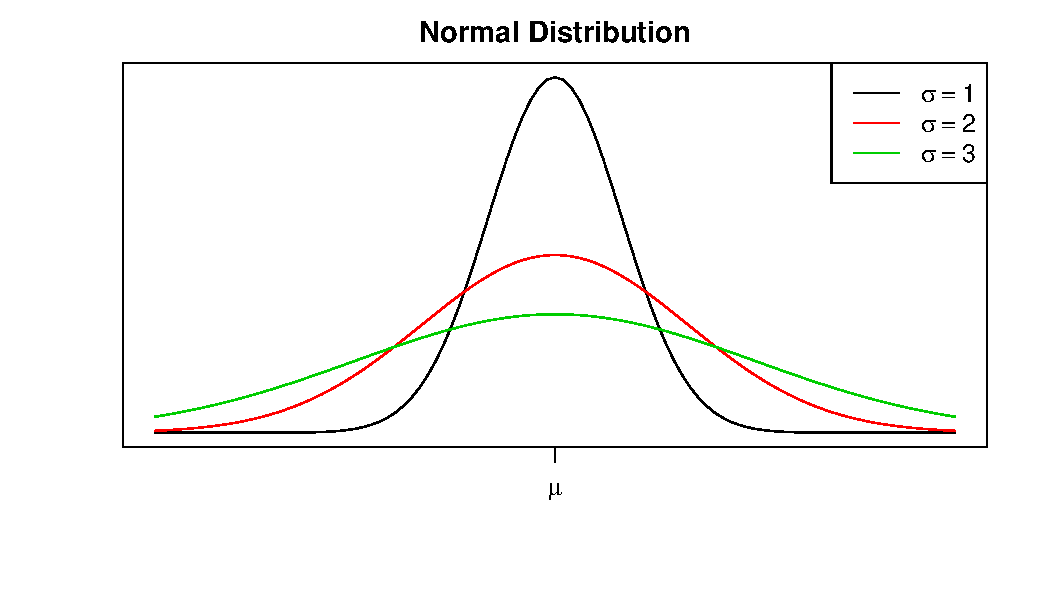
\includegraphics[width=\maxwidth]{figure/beamer-unnamed-chunk-1-1} 

}



\end{knitrout}
The tails of this distribution actually run from -$\infty$ to $\infty$.
\end{frame}

\begin{frame}[fragile]{Null Hypothesis}
\begin{itemize}
\item For the one sample problem, we may wish to test the hypothesis that the population is centered at some supposed value $\mu_0$.
\item In more statistical terms, we may wish to test the \define{null hypothesis} of  $H_0: \mu = \mu_0$.
\item In this course the null hypothesis, $H_0$, always contains a statement of no change ($=$). *This is not universal across textbooks. \nl
\end{itemize}
\end{frame}

\begin{frame}[fragile]{Alternative Hypothesis}
\begin{itemize}
\item $H_0$ is tested against a competing statement called the \define{alternative hypothesis} $H_1$ (sometimes written $H_A$).
\item We can either make this alternative one or two-sided:
\begin{itemize}
\item[] $H_1: \mu \neq \mu_0$ (two-sided)
\item[] $H_1: \mu < \mu_0$ (one-sided, lower-tailed)
\item[] $H_1: \mu > \mu_0$ (one-sided, upper-tailed)
\end{itemize}
\item $H_0$ and $H_1$ should always be written in terms of the \textit{population} parameters (in this case $\mu$).
\end{itemize}
\end{frame}



\frame{
\frametitle{Alternative Hypothesis} 

\begin{itemize}
\item  The direction of our alternative hypothesis will depend on the situation at hand.

 \item A two-sided alternative may be preferred if %you no suspicion of specific direction (i.e. $>$ or $<$ than) in advanced.\nl
 a deviation in either direction is just as grave.
\begin{itemize}
\item  eg. to compare a new medical treatment to a placebo (we care both if the treatment is effective and if it is harmful). %eg. to determine whether  monthly energy cost for families has changed from the previous year}
% \item For example, if we are trying to determine the right dose for a drug, we want to make sure we dont overmedicate (which could lead to adverse health affects) or undermedicate (which would render our drug ineffective).
\end{itemize}
\end{itemize}
}



\frame{
\frametitle{Alternative Hypothesis} 

\begin{itemize}

 \item One-sided alternatives may be preferred if %you no suspicion of specific direction (i.e. $>$ or $<$ than) in advanced.\nl
 results of your test are only relavent in one direction.
\begin{itemize}
\item eg. is this years sales better than the previous year? (if yes, employees get a bonus, if not, nothing happens) %identifying customer buying properties, online advertising optimization.
\item eg. do less than half the adults in a certain area favour the construction of an outdoor rink? %in determining %if data sets match a model, understanding scientific process based on collected data values, analysis of study data.
\end{itemize}
\end{itemize}
}


\begin{frame}[fragile]{One Sample Test Example}
\vfill
\begin{itemize}
\item A \emph{one sample test} can be used to compare a sample to a model or known population/estimate.
\vfill
\item To put another way, this test is used to determine if the sample mean $\xbar$ is significantly different then some hypothesized value $\mu_0$.
\vfill
\item As an example, using the car data test if the average mileage is different than 10km/L.
\vfill
\end{itemize}
\end{frame}
%%%%%%%%%%%%%%%%%%%%%%%%%%%%%%%%%%%%%%%%%%%%%%%%%%%%%%%%%%%%%%%%%%%%%%%%%%%%%%%%%%%%%%%%%%%%%%%%%%%%


\begin{frame}[fragile]{One Sample Test Example}
\vfill
\begin{itemize}
\item Consider the scenario where this collection of cars \textit{is} in fact sampled from a population having a mean average mileage equal to 10km/L. (i.e. our null hypothesis is correct).
\item Based on the randomness of sampling, it would be unrealistic to expect that our sample would produce an $\xbar$ exactly equal to 10km/L.\nl
\item Therefore we should expect some plausible wiggle room around our hypothesized value of 10 which we would deem close enough.\nl
\end{itemize}
\end{frame}


\begin{frame}[fragile]{One Sample Test Example}
\vfill
\begin{itemize}
\item On the contrary, once we pass a certain threshold, we could determine that our sample is inconsistent with our hypothesis. 
\item That threshold should of course depend on the problem at hand.
\item For example, we would explect the threshold for the black curve on \hyperlink{normal}{this} slide should would be more strict than the thresold for the green curve. 
\end{itemize}
\end{frame}



%%%%%%%%%%%%%%%%%%%%%%%%%%%%%%%%%%%%%%%%%%%%%%%%%%%%%%%%%%%%%%%%%%%%%%%%%%%%%%%%%%%%%%%%%%%%%%%%%%%%
\begin{frame}[fragile]{One Sample Test: Hypotheses Statements}
\begin{itemize}
% \item  Alternatively hypothesis ($H_A$) can be one sided ($<$ or $>$) or two sided ($\neq$).
% \begin{align*}
% H_0: \mu = \mu_0& \quad vs  &H_A: \mu > \mu_0
% \end{align*}
% \vfill
\item In the car mileage example, we are testing:
\begin{align*}
H_0: \mu = 10& \quad vs  &H_1: \mu \neq 10
\end{align*}
that is to say, our hypothesized value is $\mu_0 = 10$.
\item Analogous to the courtroom, we believe $H_0$ is true until evidence (in the form of data) suggests otherwise.
\item To determine our threshold which determines how far our sample mean needs to depart from 10 before we no longer believe $H_0$ is true, we need a \define{test statistic}.  
%More generically, we use $H_0: \mu = \mu_0$ where $\mu_0$ is the hypothesized mean.
\vfill
\end{itemize}
\end{frame}
%%%%%%%%%%%%%%%%%%%%%%%%%%%%%%%%%%%%%%%%%%%%%%%%%%%%%%%%%%%%%%%%%%%%%%%%%%%%%%%%%%%%%%%%%%%%%%%%%%%%


%%%%%%%%%%%%%%%%%%%%%%%%%%%%%%%%%%%%%%%%%%%%%%%%%%%%%%%%%%%%%%%%%%%%%%%%%%%%%%%%%%%%%%%%%%%%%%%%%%%%
\begin{frame}[fragile]{One Sample Test: Calculate Test Statistic}
\vfill
For the one sample test the $t$-test statistic is calculated as:
\begin{equation}\label{teststat}
t = \dfrac{\xbar - \mu_0}{\dfrac{s}{\sqrt n}}
\end{equation}
\vfill
$\xbar$ is a sample mean, $s$ is sample standard deviation, $n$ is sample size, $\mu_0$ is hypothesized mean value
\vfill
As alluded to eariler, this statistic follows a $t$-distribution.
\end{frame}

\begin{frame}[fragile]
The distribution of \eqref{teststat} looks like this:
\begin{knitrout}\footnotesize
\definecolor{shadecolor}{rgb}{0.969, 0.969, 0.969}\color{fgcolor}

{\centering 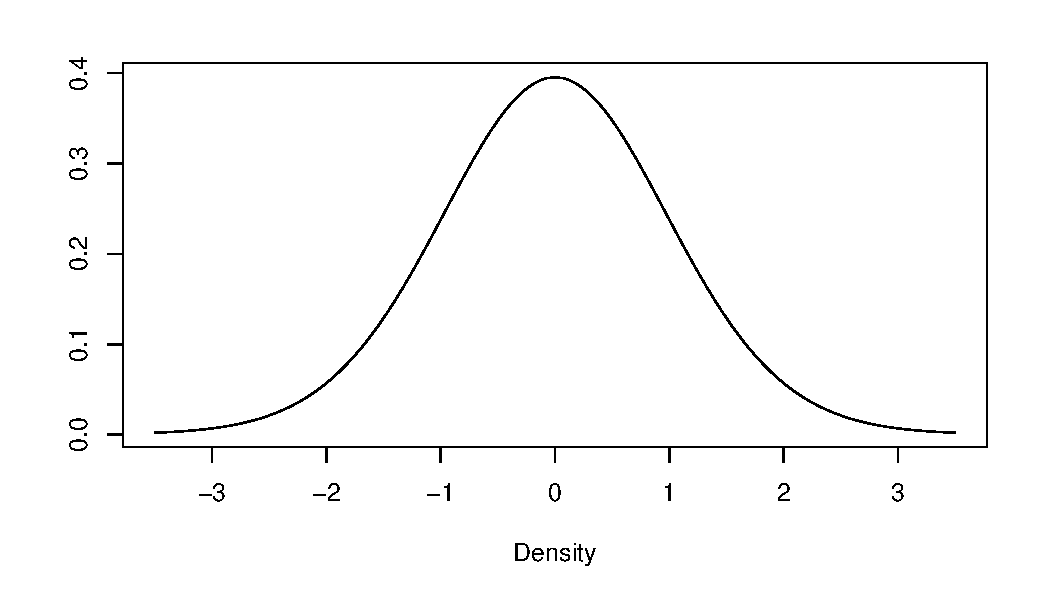
\includegraphics[width=\maxwidth]{figure/beamer-unnamed-chunk-2-1} 

}



\end{knitrout}

\end{frame}

\begin{frame}[fragile]
\begin{knitrout}\footnotesize
\definecolor{shadecolor}{rgb}{0.969, 0.969, 0.969}\color{fgcolor}

{\centering 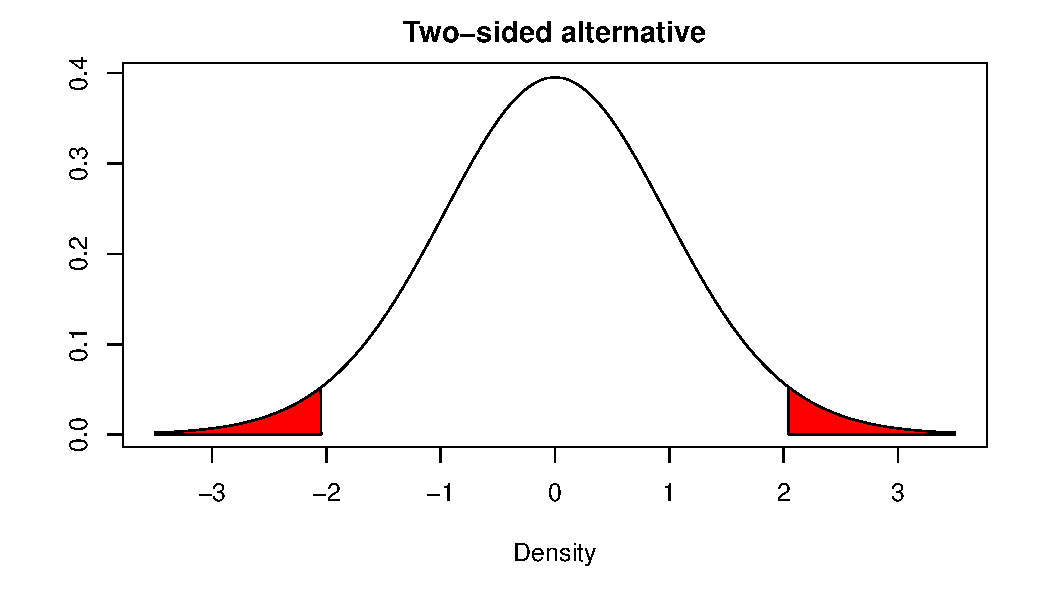
\includegraphics[width=\maxwidth]{figure/beamer-unnamed-chunk-3-1} 

}



\end{knitrout}
\end{frame}

\begin{frame}[fragile]
\begin{itemize}
\item If the hypothesis is true, there is only a 5\% chance that our test statistic falls in the area in red.  
\item This may seem like a reasonable way to determine our threshold for believing $H_0: \mu = 10$. 

 \item To put numbers to this example, if $\xbar$ is less than -9.6446667 or bigger than 10.3553333 we will no longer believe the null hypothesis that the average gas mileage for this population of cars is equal to 10km/L. 
\end{itemize}
\end{frame}

\begin{frame}[fragile]
\begin{itemize}
\item Indeed this line of thinking is exactly what we follow when forming conclusions for a \textit{two-sided} \rf{t.test}. 
\item  A similar argument can be made for one-sided tests:
\vfill
\begin{knitrout}\footnotesize
\definecolor{shadecolor}{rgb}{0.969, 0.969, 0.969}\color{fgcolor}

{\centering 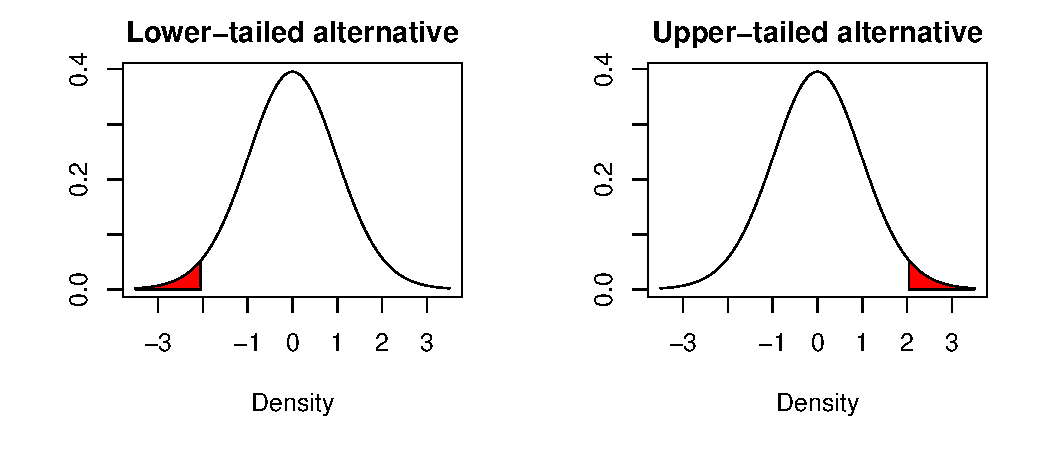
\includegraphics[width=\maxwidth]{figure/beamer-unnamed-chunk-5-1} 

}



\end{knitrout}
\item This area in red is sometimes referred to as the \define{rejection region}.
\end{itemize}
\end{frame}

\begin{frame}{Hypothesis testing in R}
\begin{itemize}
\item Now that we have an understanding of what these tests are doing, lets see how we can code them up in R. 
\item The general syntax for performing t.test in R is:
\begin{center}
\rt{\rf{t.test}(\rp{x}=mydata,\rp{alternative}="two.sided",\rp{mu} =} $\mu_0$ \rt{,\rp{conf.level}=0.95,...,)}
\end{center}
\item In R the default \rp{alterative} is \ro{"two.sided"} with the options \ro{"less"}, or \ro{"greater"}.
\item As usually, to see the help file on this function, we type \rt{?t.test}.

\end{itemize}
\end{frame}


\begin{frame}{Hypothesis testing in R}
\begin{itemize}
\item The \rp{conf.level} = 1 - $\alpha$, where $\alpha$ denotes our significance level.
\item The \define{significance level} determines how much of the probability we allow in the rejection region.  
\item Typically $\alpha = 5\%$ so that the \rp{conf.level} = 95\% (or 0.95)
\item A confidence level of 0.95 is the default setting in R, hence we will usually not specify it in the code to follow.
\end{itemize}
\end{frame}



\begin{frame}[fragile]{One Sample Test: Cars Example}
The following code will  perform a one-sample $t$-test which tests:
\begin{align*}
H_0: \mu = 10& \quad \quad vs  &H_1: \mu \neq 10
\end{align*}
\begin{knitrout}\footnotesize
\definecolor{shadecolor}{rgb}{0.969, 0.969, 0.969}\color{fgcolor}\begin{kframe}
\begin{alltt}
\hlstd{car_data} \hlkwb{<-} \hlkwd{read.csv}\hlstd{(}\hlstr{"car_data.csv"}\hlstd{)}\hlcom{# read in the data}
\hlkwd{t.test}\hlstd{(}\hlkwc{x}\hlstd{=car_data}\hlopt{$}\hlstd{km.L,}             \hlcom{# sample mileage}
       \hlkwc{alternative}\hlstd{=}\hlkwd{c}\hlstd{(}\hlstr{"two.sided"}\hlstd{),}  \hlcom{# two-side H_A}
       \hlkwc{mu}\hlstd{=}\hlnum{10}\hlstd{)} \hlcom{# set the hypothesized value equal to 10. }

\hlcom{# since a two-sided test is the default, we could have typed:}
\hlkwd{t.test}\hlstd{(}\hlkwc{x}\hlstd{=car_data}\hlopt{$}\hlstd{km.L,} \hlkwc{mu}\hlstd{=}\hlnum{10}\hlstd{)}
\end{alltt}
\end{kframe}
\end{knitrout}
% \begin{Verbatim}[xleftmargin=2em, xrightmargin=1.5em, frame=single, label=R code, framesep=0.5em]
% car_data <- read.csv("car_data.csv")
% t.test(x=car_data$km.L,
%        alternative=c("two.sided"), mu=10)
% \end{Verbatim}
\end{frame}
%%%%%%%%%%%%%%%%%%%%%%%%%%%%%%%%%%%%%%%%%%%%%%%%%%%%%%%%%%%%%%%%%%%%%%%%%%%%%%%%%%%%%%%%%%%%%%%%%%%%



\begin{frame}[fragile]{R Output}
\begin{knitrout}\footnotesize
\definecolor{shadecolor}{rgb}{0.969, 0.969, 0.969}\color{fgcolor}\begin{kframe}
\begin{verbatim}
## 
## 	One Sample t-test
## 
## data:  car_data$km.L
## t = 1.608, df = 29, p-value = 0.1187
## alternative hypothesis: true mean is not equal to 10
## 95 percent confidence interval:
##   9.90338 10.80729
## sample estimates:
## mean of x 
##  10.35533
\end{verbatim}
\end{kframe}
\end{knitrout}
\end{frame}


\begin{frame}[fragile]{Decision and Conclusion (using $P$-value)}
\vfill
\begin{itemize}
\item In order to make a conclusion based on this output, we usually look at a $p$-value.
\item The \define{p-value}, is the probability of sampling data more extreme than what we observed when the null hypothesis $H_0$ is true.
\item Hence the smaller this value is, the more unlikely our null hypothesis is true.
\end{itemize}
\end{frame}



\begin{frame}
\begin{itemize}
\item {\bf Question}: How small is \textit{too small}? 
\begin{itemize}
\item {\bf Answer}: Anything less that the significance level $\alpha$, we deem too small.
\end{itemize}
\item  {\bf Why?} This $p$-value has a one-to-one relationship with the rejection region method described earlier.
\item To be more specific, if our sample surpasses our threshold, the $p$-value will necessarily be less than $\alpha$.
\end{itemize}
\end{frame}


%%%%%%%%%%%%%%%%%%%%%%%%%%%%%%%%%%%%%%%%%%%%%%%%%%%%%%%%%%%%%%%%%%%%%%%%%%%%%%%%%%%%%%%%%
\begin{frame}[fragile]{Decision and Conclusion (using $P$-value)}
Assuming our $\alpha$/significance level is 5\%\dots
\vfill
If \alert{$p{\rm-value} > 0.05$}, the probability of seeing a sample mean more extreme than $\xbar$ is not that unlikely.
\vfill
Our decision/conclusion would be:
\begin{enumerate}
\item \alert{Fail to reject the null hypothesis}.
\item There is insufficient  evidence to suggest that the mean value is less than/greater than/different than the test value (will depend on alternative hypothesis)
\end{enumerate}
\end{frame}

\begin{frame}[fragile]{Decision and Conclusion (using $P$-value)}
\vfill

If \alert{$p{\rm-value} < 0.05$}, the probability of seeing a sample mean more exteme than $\xbar$ is unlikely.

\vfill
Our decision/conclusion would be:
\begin{enumerate}
\item \alert{Reject the null hypothesis}.
\item There is statistically significant evidence to suggest that the mean value is less than that/greater than/ different than the test value  (will depend on alternative hypothesis).
\end{enumerate}
\vfill
\end{frame}
%%%%%%%%%%%%%%%%%%%%%%%%%%%%%%%%%%%%%%%%%%%%%%%%%%%%%%%%%%%%%%%%%%%%%%%%%%%%%%%%%%%%%%%%%

\begin{frame}[fragile]{Under the hood calculations}

\begin{itemize}
\item Returning to our car example, recall that we are testing:
 \begin{itemize}
 \item $H_0: \mu = 10$ vs. $H_1: \mu \neq 10$.
 \end{itemize}
\item Intuitively, as our sample mean $\xbar$ gets father and rather away from 10, this would indicate stronger and stronger evidence against the null hypothesis.
 \item We can see calculate our test statistic:
\begin{equation*}
 \dfrac{\xbar - \mu_0}{\dfrac{s}{\sqrt n}} =
 \dfrac{10.3553333 - 10}{\dfrac{1.210354}{\sqrt 30}}
 ={1.6079931}
 \end{equation*}
 and find the corresponding $p$-value = \emph{0.11867}.
\end{itemize}
\end{frame}


\begin{frame}[fragile]{Two sided test}
For the visual learners, we can view our $p$-value as follows:
\begin{knitrout}\footnotesize
\definecolor{shadecolor}{rgb}{0.969, 0.969, 0.969}\color{fgcolor}

{\centering 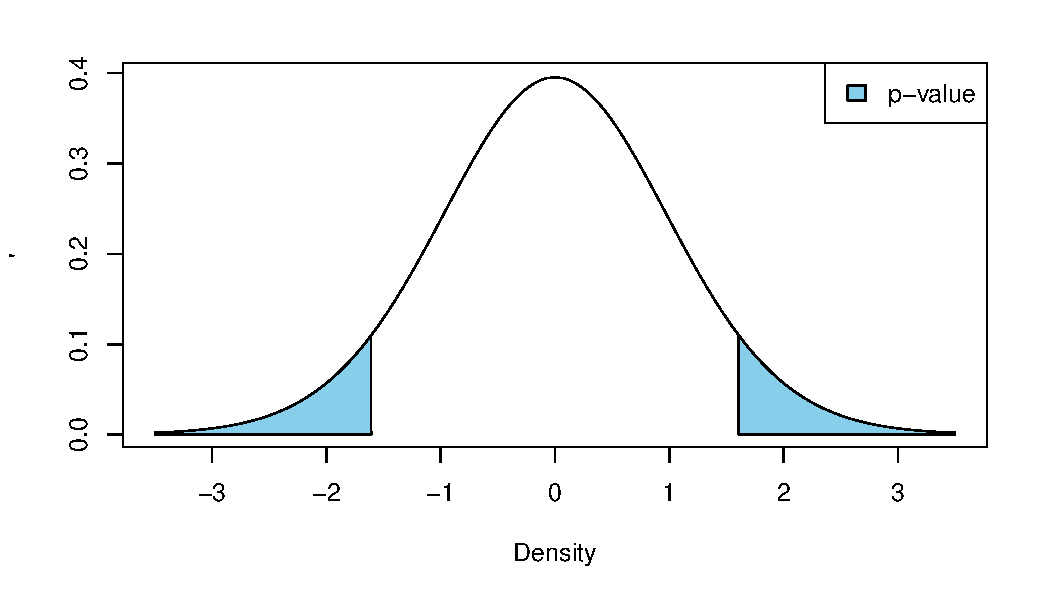
\includegraphics[width=0.8\linewidth]{figure/beamer-unnamed-chunk-8-1} 

}



\end{knitrout}
\end{frame}


\begin{frame}[fragile]
\begin{knitrout}\footnotesize
\definecolor{shadecolor}{rgb}{0.969, 0.969, 0.969}\color{fgcolor}

{\centering 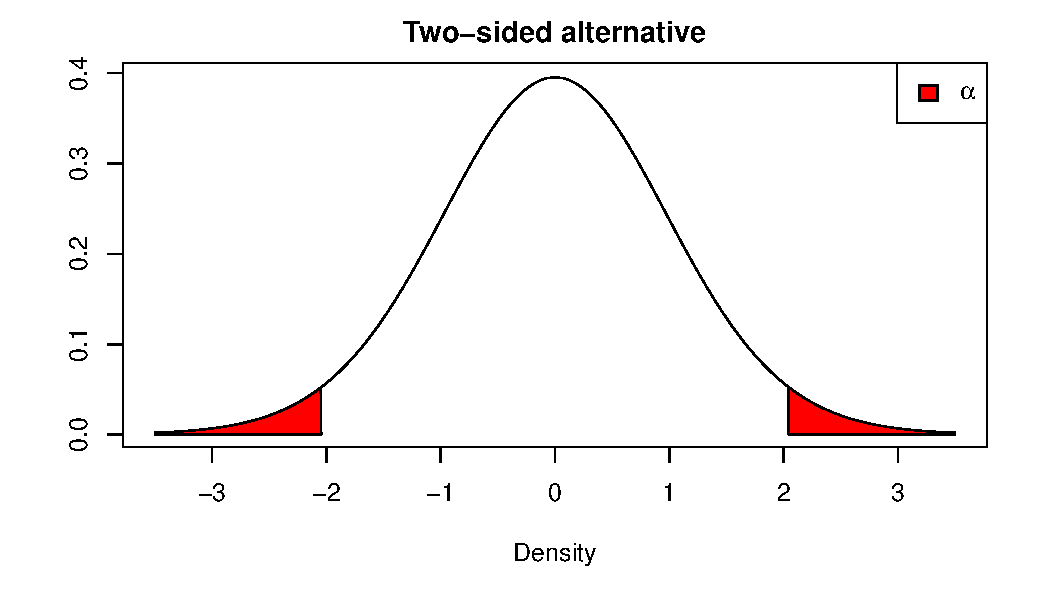
\includegraphics[width=\maxwidth]{figure/beamer-unnamed-chunk-9-1} 

}



\end{knitrout}
\end{frame}



\begin{frame}{Alternative ways of thinking}
\begin{itemize}
\item Since this blue area on the previous slide makes up more than 5\%, we fail to reject the null hypothesis.
\item Since the probability of observing a sample mean more extreme than the one we saw (i.e $> 10.355$ or $< -10.355$) is quite likely (approximate 11.9\%), we fail to reject the null hypothesis.
\end{itemize} 
\end{frame}

%%%%%%%%%%%%%%%%%%%%%%%%%%%%%%%%%%%%%%%%%%%%%%%%%%%%%%%%%%%%%%%%%%%%%%%%%%%%%%%%%%%%%%%%%%%%%%%%%%%%

%%%%%%%%%%%%%%%%%%%%%%%%%%%%%%%%%%%%%%%%%%%%%%%%%%%%%%%%%%%%%%%%%%%%%%%%%%%%%%%%%%%%%%%%%%%%%%%%%%%%
\begin{frame}[fragile]{Decision and Conclusions (using $P$-value)}

\begin{itemize}
\item While it is important to understand the ``under-the-hood calculations" (see STAT 230 for more) all of our decisions for this course may be based on the R output.  
\vfill
\item Since the $p$-value of $0.11867$ is greater than our significance level of 0.05, we \emph{ fail to reject the null hypothesis}.
\vfill
\end{itemize}
\end{frame}


\begin{frame}[fragile]{R output:}
\begin{Verbatim}[xleftmargin=2em, xrightmargin=1.5em, frame=single, label=R code, framesep=0.5em, fontsize=\small, commandchars=\\\{\}]
> t.test(x=car_data$km.L, mu=10)
            
            One Sample t-test
            
data: car_data$km.L
t = 1.608, df = 29, \emph{p-value = 0.1187}
alternative hypothesis: true mean is not equal to 10
95 percent confidence interval:
    9.90338  10.80729
sample estimates:
mean of x
  10.35533
\end{Verbatim}
\end{frame}
%%%%%%%%%%%%%%%%%%%%%%%%%%%%%%%%%%%%%%%%%%%%%%%%%%%%%%%%%%%%%%%%%%%%%%%%%%%%%%%%%%%%%%%%%%%%%%%%%%%%




\begin{frame}[fragile]{Decision and Conclusions (using $P$-value)}
\begin{itemize}
\item We usually like to state our conclusions in terms of the problem at hand,\dots
\vfill
\item Hence, there is insufficient evidence to suggest that the mean mileage differs from 10 km/L.
\vfill
\item N.B: We \red{never} claim that either the null or alternative hypothesis is true.  We can only ``reject" or ``fail to reject" the null hypothesis.
\vfill
\end{itemize}
\end{frame}
%%%%%%%%%%%%%%%%%%%%%%%%%%%%%%%%%%%%%%%%%%%%%%%%%%%%%%%%%%%%%%%%%%%%%%%%%%%%%%%%%%%%%%%%%%%%%%%%%%%%

\begin{frame}
\begin{itemize}
\item Before moving on to the two-sample problem, it is worth discussing the \define{confidence interval} which is also produced as output for a $t$-test.\nl
\item This interval gives us a range of plausible values for $\mu$ (regardless of our hypothesized value $\mu_0$)
\end{itemize}
\end{frame}

\begin{frame}[fragile]
\vfill
\begin{block}{General Form of Confidence Interval (CI):}
The general form of a confidence interval looks like this:
\begin{align*}
\text{point estimate }&\pm \text{ margin of error}\\
(\hat\mu-m.e.&,\, \hat\mu+m.e.)
\end{align*}
\end{block}
{\bf Interpretation:} Assuming a confidence level of 95\%, we are 95\% confident that the interval will contain the true value of the parameter.
\vfill
\end{frame}



%%%%%%%%%%%%%%%%%%%%%%%%%%%%%%%%%%%%%%%%%%%%%%%%%%%%%%%%%%%%%%%%%%%%%%%%%%%%%%%%%%%%%%%%
\begin{frame}[fragile]{Decision and Conclusions (using CI)}\small
\begin{Verbatim}[xleftmargin=2em, xrightmargin=1.5em, frame=single, label=R code, framesep=0.5em, fontsize=\footnotesize, commandchars=\\\{\}]
> t.test(x=car_data$km.L, mu=10)
            One Sample t-test
data: car_data$km.L
t = 1.608, df = 29, p-value = 0.1187
alternative hypothesis: true mean is not equal to 10
\emph{95 percent confidence interval:}
\emph{    9.90338  10.80729}
sample estimates:
mean of x
  10.35533
\end{Verbatim}
\end{frame}
%%%%%%%%%%%%%%%%%%%%%%%%%%%%%%%%%%%%%%%%%%%%%%%%%%%%%%%%%%%


\begin{frame}
When the input argument \rt{\rp{conf.level}=0.95} = (1-$\alpha$) in the \rf{t.test} function, a 95\% confidence interval is produce. \nl
Other not-so-typical alternatives might be:
\begin{itemize}
\item setting \rt{\rp{conf.level}=0.90}, and obtaining a 90\% confidence interval.
\item setting \rt{\rp{conf.level}=0.98}, and obtaining a 98\% confidence interval.
\item setting \rt{\rp{conf.level}=0.99}, and obtaining a 99\% confidence interval.
\end{itemize}
\end{frame}


\begin{frame}
\begin{itemize}
\item We can actually make a conclusion (reject or fail to reject) based on the confidence interval instead of looking at the $p$-value. \nl
\item For the car example, we are 95\% confident that the true mean mileage of the car lies within the bounds $[9.903, 10.807]$.\nl
\item Since 10 is within those bounds, the hypothesis that $\mu = 10$ would appear reasonable; hence we fail to reject $H_0$.
\vfill
\item If, for example, our CI was $[15.3, 16.4]$ instead, this hypothesis is not within reason and we would  reject the null hypothesis. 
\end{itemize}
\end{frame}

%%%%%%%%%%%%%%%%%%%%%%%%%%%%%%%%%%%%%%%%%

% \begin{frame}[fragile]{Confidence Intervals}
% Consider the following statement
% \begin{quotation}
% ``62\% of US college students miss a class due to excessive drinking.  The result is accurate with 1.7 percentage points 19 times out of 20.''
% \end{quotation}
% \vfill
% Unpacking this statement:
% \begin{enumerate}
% \item \emph{62} is the estimated percentage.
% \item \emph{1.7} is the margin of error.
% \item \emph{19 times out of 20} is the stated confidence and $100\% \frac{19}{20} = 95\%$.
% \end{enumerate}
% \vfill
% We call this a \emph{95\% confidence interval}: $(60.3,\, 63.7)$
% \vfill
% \end{frame}
%%%%%%%%%%%%%%%%%%%%%%%%%%%%%%%%%%%%%%%%%%%%%%%%%%%%%%%%%%%%%%%%%%%%%%%%%%%%%%%%%%%%%%%%%%%%%%%%%%%%

\begin{frame}{Two-sample $t$-tests}
\begin{itemize}
\item The one-sample $t$-test deals with making inference on a single sample for a single population of interest.\nl
\item Often we are concerned with \textit{two} samples from potentially different population distributions.\nl
\item The goal of a two-sampled $t$-test is usually to test the hypothesis that two samples may be assumed to come from distributions with the same mean. \nl
\end{itemize}
\end{frame}



\begin{frame}
\begin{itemize}
\item In more statistical words, if we use $\mu_A$ and $\mu_B$ to denote the true population mean of group A and group B, respectively, we may want to test whether:
\begin{align*}
H_0: \mu_A = \mu_B& \quad vs  &H_1: \mu_A \neq \mu_B
\end{align*}
\item An equivalent way of saying this is:
\begin{align*}
H_0: \mu_A - \mu_B = 0 & \quad vs  &H_1: \mu_A -  \mu_B \neq  0
\end{align*}
\item  More generically, we could test:
\begin{align*}
H_0: \mu_d = d_0 & \quad vs  &H_1: \mu_d \neq  d_0
\end{align*}
where $d_0$ is our hypothesize value for the $\mu_d$ mean \textit{difference} between group A and B. 
\end{itemize}
\end{frame}
%%%%%%%%%%%%%%%%%%%%%%%%%%%%%%%%%%%%%%%%%%%%%%%%%%%%%%%%%%%%%%%%%%%%%%%%%%%%%%%%%%%%%%%%%%%%%%%%%%%%
%%%%%%%%%%%%%%%%%%%%%%%%%%%%%%%%%%%%%%%%%%%%%%%%%%%%%%%%%%%%%%%%%%%%%%%%%%%%%%%%%%%%%%%%%%%%%%%%
\begin{frame}{Two-sample $t$-tests}
\begin{itemize}
\item Two-sampled $t$-test can actually be broken into two categories:
\begin{enumerate}
\item paired
\item unpaired
\end{enumerate}
\item \define{paired} data occur when we are obtaining two measurements on the \textit{same} individual.  Eg. midterm 1 mark and midterm 2 mark for each student in Data 301.
\item \define{unpaired} data occur when we have two \textit{independent} samples.
\end{itemize}
\end{frame}

\begin{frame}{Two-sample $t$-tests}
\begin{itemize}
\item In either case, we are still interested in comparing the group means.\nl
\item The only difference in terms of R-code is that we will need to specify \rt{\rp{paired} = TRUE} when the data are paired.\nl
\item N.B. for unpaired data we can set \rt{\rp{paired} = FALSE}, but since this is the default setting in R, this specification may be omitted from our code. 
\end{itemize}
\end{frame}



%%%%%%%%%%%%%%%%%%%%%%%%%%%%%%%%%%%%%%%%%%%%%%%%%%%%%%%%%%%%%%%%%%%%%%%%%%%%%%%%%%%%%%%%%%%%%%%%%%%%
\begin{frame}[fragile]{Two Sample Unpaired}
\vfill
An unpaired (independent) \emph{two sample test} compares two independent samples to determine if there is a difference between the groups.
\vfill
\begin{example}
\begin{enumerate}
\item Compare effectiveness of two different drugs tested on two sets of patients.\\
\item Experiment versus control samples.
\end{enumerate}
\end{example}
\vfill
\end{frame}
%%%%%%%%%%%%%%%%%%%%%%%%%%%%%%%%%%%%%%%%%%%%%%%%%%%%%%%%%%%%%%%%%%%%%%%%%%%%%%%%%%%%%%%%%%%%%%%%%%%%


%%%%%%%%%%%%%%%%%%%%%%%%%%%%%%%%%%%%%%%%%%%%%%%%%%%%%%%%%%%%%%%%%%%%%%%%%%%%%%%%%%%%%%%%%%%%%%%%%%%%
\begin{frame}[fragile]{Two Sample Unpaired Example}
{Hypothesis Statement}
Using the \verb|beaver2| dataset in R, test the hypothesis that there is no difference between the average temperature of active beavers and non-active beavers.\nl
Letting 
$\mu_1$ and $\mu_2$ represent the mean temperatures of active and non-active beavers, respectively, our hypotheses may be written:
\begin{align*}
H_0 : \mu_1 -\mu_2 =0 \to \mu_d = 0 \quad vs. \quad H_1:\mu_1 - \mu_2  = 0 \to \mu_d \neq 0
\end{align*}
N.B. we can change the hypothesized value  $\mu_0 = 0$ to any value and the choice of an upper/lower-tailed alternative.
\end{frame}
%%%%%%%%%%%%%%%%%%%%%%%%%%%%%%%%%%%%%%%%%%%%%%%%%%%%%%%%%%%%%%%%%%%%%%%%%%%%%%%%%%%%%%%%%%%%%%%%%%%%


\begin{frame}{Hypothesis testing in R}{Unpaired two-sample $t$-test}
\begin{itemize}
\item The general syntax for performing an unpaired two-sample t.test in R is:
\begin{center}
\rt{\rf{t.test}(\rp{x}=A, \rp{y}=B,\rp{alternative}="two.sided",\rp{mu} =} $d_0$ \rt{,\rp{conf.level}=0.95, \rp{data}=\ro{mydata}, \dots)}
\end{center}
\item Alternatively, we could specify a \textit{formula}
\begin{center}
\rt{\rf{t.test}(\rp{formula}=A$\sim$B,\rp{alternative}="two.sided",\rp{mu} =} $d_0$ \rt{,\rp{conf.level}=0.95, \rp{data}=\ro{mydata}, \dots)}
\end{center}
\item Where \ro{A} and \ro{B} contain the samples from group A and B, respectively.
\end{itemize}
\end{frame}


%%%%%%%%%%%%%%%%%%%%%%%%%%%%%%%%%%%%%%%%%%%%%%%%%%%%%%%%%%%%%%%%%%%%%%%%%%%%%%%%%%%%
\begin{frame}[fragile]{Two Sample Unpaired Example}
Lets have a look at the {\tt beaver2} data:
\begin{knitrout}\footnotesize
\definecolor{shadecolor}{rgb}{0.969, 0.969, 0.969}\color{fgcolor}\begin{kframe}
\begin{alltt}
\hlkwd{head}\hlstd{(beaver2,}\hlnum{3}\hlstd{)}
\end{alltt}
\begin{verbatim}
##   day time  temp activ
## 1 307  930 36.58     0
## 2 307  940 36.73     0
## 3 307  950 36.93     0
\end{verbatim}
\begin{alltt}
\hlkwd{tail}\hlstd{(beaver2,}\hlnum{3}\hlstd{)}
\end{alltt}
\begin{verbatim}
##     day time  temp activ
## 98  308  140 38.01     1
## 99  308  150 38.04     1
## 100 308  200 38.07     1
\end{verbatim}
\end{kframe}
\end{knitrout}
\end{frame}
%%%%%%%%%%%%%%%%%%%%%%%%%%%%%%%%%%%%%%%%%%%%%%%%%%%%%%%%%%%%%%%%%%%%%%%%%%%%%%%%%%%%%


\begin{frame}[fragile]{Two Sample Unpaired Example}
\begin{itemize}
\item  As seen in the help file \rt{?beaver2} the {\tt activ} variable denotes activity level of the beaver (1 = active, 0=non-active)
\item We could create a subset of this data and perform a t-test as follows:
\end{itemize}
\begin{knitrout}\footnotesize
\definecolor{shadecolor}{rgb}{0.969, 0.969, 0.969}\color{fgcolor}\begin{kframe}
\begin{alltt}
\hlstd{beaverA} \hlkwb{<-} \hlkwd{subset}\hlstd{(beaver2, activ}\hlopt{==}\hlnum{1}\hlstd{)} \hlcom{#active beavers}
\hlstd{beaverB} \hlkwb{<-} \hlkwd{subset}\hlstd{(beaver2, activ}\hlopt{==}\hlnum{0}\hlstd{)} \hlcom{#non-active beavers}
\hlkwd{t.test}\hlstd{(beaverA}\hlopt{$}\hlstd{temp, beaverB}\hlopt{$}\hlstd{temp)}
\end{alltt}
\end{kframe}
\end{knitrout}
\end{frame}

\begin{frame}[fragile]\label{explicit}
To see the more verbose specification:
\begin{knitrout}\footnotesize
\definecolor{shadecolor}{rgb}{0.969, 0.969, 0.969}\color{fgcolor}\begin{kframe}
\begin{alltt}
\hlkwd{t.test}\hlstd{(beaverA}\hlopt{$}\hlstd{temp,} \hlcom{# temperatures of 62 active beavers}
       \hlstd{beaverB}\hlopt{$}\hlstd{temp,} \hlcom{# temps of 38 inactive beavers}
       \hlkwc{alternative} \hlstd{=} \hlstr{"two.sided"}\hlstd{,} \hlcom{# H_1: mu_A - mu_B != d_0}
       \hlkwc{mu} \hlstd{=} \hlnum{0}\hlstd{,}                    \hlcom{# default d_0 = 0}
       \hlkwc{paired} \hlstd{=} \hlnum{FALSE}\hlstd{,}            \hlcom{# default (data unpaired)}
       \hlkwc{conf.level} \hlstd{=} \hlnum{0.95}          \hlcom{# default (ie. alpha = 5%)}
       \hlstd{)}
\end{alltt}
\end{kframe}
\end{knitrout}

\end{frame}

\begin{frame}[fragile]
{R output}
\begin{knitrout}\footnotesize
\definecolor{shadecolor}{rgb}{0.969, 0.969, 0.969}\color{fgcolor}\begin{kframe}
\begin{verbatim}
## 
## 	Welch Two Sample t-test
## 
## data:  beaverA$temp and beaverB$temp
## t = 18.548, df = 80.852, p-value < 2.2e-16
## alternative hypothesis: true difference in means is not equal to 0
## 95 percent confidence interval:
##  0.7197342 0.8927106
## sample estimates:
## mean of x mean of y 
##  37.90306  37.09684
\end{verbatim}
\end{kframe}
\end{knitrout}
\end{frame}

\begin{frame}[fragile]{Two Sample Unpaired Example}\label{formula}
Alternatively we could have used the formula option:
\begin{knitrout}\footnotesize
\definecolor{shadecolor}{rgb}{0.969, 0.969, 0.969}\color{fgcolor}\begin{kframe}
\begin{alltt}
\hlkwd{t.test}\hlstd{(temp}\hlopt{~}\hlstd{activ,} \hlkwc{data}\hlstd{=beaver2)}
\end{alltt}
\end{kframe}
\end{knitrout}
This tells R that the relevant data appear in the \ro{temp} column of data.frame \ro{beaver2} and that the these samples should be divided according to the factor \ro{active}.\nl
Both options should produce identical $p$-values.\footnote{test statistic may change sign depending }
\end{frame}


\begin{frame}[fragile]{Two Sample Unpaired Example}
\begin{knitrout}\footnotesize
\definecolor{shadecolor}{rgb}{0.969, 0.969, 0.969}\color{fgcolor}\begin{kframe}
\begin{alltt}
\hlstd{(bsum} \hlkwb{<-} \hlkwd{t.test}\hlstd{(temp}\hlopt{~}\hlstd{activ,} \hlkwc{data}\hlstd{=beaver2))}
\end{alltt}
\begin{verbatim}
## 
## 	Welch Two Sample t-test
## 
## data:  temp by activ
## t = -18.548, df = 80.852, p-value < 2.2e-16
## alternative hypothesis: true difference in means is not equal to 0
## 95 percent confidence interval:
##  -0.8927106 -0.7197342
## sample estimates:
## mean in group 0 mean in group 1 
##        37.09684        37.90306
\end{verbatim}
\end{kframe}
\end{knitrout}
\end{frame}



\begin{frame}[fragile]{Footnote}
\begin{itemize}
\item As we are only interested in the $p$-value, you shouldn't be bothered that the test statistic changed signs depending on how we coded this up in R.
\item But in case you are wondering, the \hyperlink{explicit}{explicit} notation is testing:
\begin{align*}
H_0 : \mu_1 -\mu_2 = 0 \quad vs. \quad H_1:\mu_1 - \mu_2 \neq 0
\end{align*}
whereas the \hyperlink{formula}{formula}  notation is testing: 
\begin{align*}
H_0 : \mu_{\red{2}} -\mu_{\red{1}} = 0 \quad vs. \quad H_1:\mu_{\red{2}} - \mu_{\red{1}} \neq 0
\end{align*}
\item For two-sided alternatives this matters not, but for one-sided tests, we need to pay close attention to the direction of $<$/$>$.
\end{itemize}
\end{frame}

\begin{frame}[fragile]
To produce output identical to the \hyperlink{formula}{formula} notation use:
\begin{knitrout}\footnotesize
\definecolor{shadecolor}{rgb}{0.969, 0.969, 0.969}\color{fgcolor}\begin{kframe}
\begin{alltt}
\hlcom{# places inactive beavers in the first argument: }
\hlkwd{t.test}\hlstd{(beaverB}\hlopt{$}\hlstd{temp,beaverA}\hlopt{$}\hlstd{temp)}
\end{alltt}
\begin{verbatim}
## 
## 	Welch Two Sample t-test
## 
## data:  beaverB$temp and beaverA$temp
## t = -18.548, df = 80.852, p-value < 2.2e-16
## alternative hypothesis: true difference in means is not equal to 0
## 95 percent confidence interval:
##  -0.8927106 -0.7197342
## sample estimates:
## mean of x mean of y 
##  37.09684  37.90306
\end{verbatim}
\end{kframe}
\end{knitrout}

\end{frame}

% \begin{frame}[fragile]{Two Sample Unpaired Example}
% \begin{itemize}
% \item As we are only interested in the $p$-value, you shouldn't be bothered that the test statistic changed signs depending on how we coded this up in R.
% \item But in case you are wondering, \hlink{formula}{formula notation} is testing:
% \begin{align*}
% H_0 : \mu_1 -\mu_2 = 0 \quad vs. \quad H_1:\mu_1 - \mu_2 \neq 0
% \end{align*}
% where as the 
% \end{itemize}
% \end{frame}

\begin{frame}
\begin{itemize}
\item Based on the $p$-value provided in the summary = \ensuremath{7.2691124\times 10^{-31}}
, there is very strong evidence to suggest that the average temperature between active and non-active beavers are different from one another.
\item We can use the language of ``strong" since the $p$-value is so small.
\item Note that we still  have the relationship between the two-sided test and the corrresponding confidence interval.
\item The CI is highlighted in pink in the following slide \dots
\end{itemize}
\end{frame}




%%%%%%%%%%%%%%%%%%%%%%%%%%%%%%%%%%%%%%%%%%%%%%%%%%%%%%%%%%%%%%%%%%%%%%%%%%%%%%%%%%%%%%%%%%%%%%%%%%%%
\begin{frame}[fragile]{Two Sample Unpaired Example}
\begin{Verbatim}[xleftmargin=2em, xrightmargin=1.5em, frame=single, label=Using CI-value, framesep=0.5em, commandchars=\\\{\}, fontsize=\footnotesize]
> t.text(temp-activ, data=beaver2, alternative=c("two.sided"), mu=0,
paired=FALSE)
        welch Two Sample t-test
data:    temp by activ
t = -18.548,  df = 80.852, p-value < 2.2e-16
alternative hypothesis: true difference in means is not equal to 0
95 percent condifence interval:
  \emph{-0.8927106  -0.7197342}
sample estimates:
mean in group 0 mean in group 1
       37.09684        37.90306
\end{Verbatim}

\vfill
\end{frame}
%%%%%%%%%%%%%%%%%%%%%%%%%%%%%%%%%%%%%%%%%%%%%%%%%%%%%%%%%%%%%%%%%%%%%%%%%%%%%%%%%%%%%%%%%%%%%%%%%%%%


% %%%%%%%%%%%%%%%%%%%%%%%%%%%%%%%%%%%%%%%%%%%%%%%%%%%%%%%%%%%%%%%%%%%%%%%%%%%%%%%%%%%%%%%%%%%%%%%%%%%%
% \begin{frame}[fragile]{Two Sample Unpaired Example Test Statistic}
% \vfill
% Use $t$-test statistics.
% \vfill
% \begin{Verbatim}[xleftmargin=2em, xrightmargin=1.5em, frame=single, numbers=left, label=Using P-value, framesep=0.5em, commandchars=\\\{\}]
% # Need to set active to be a factor first.
% beaver2$activ = as.factor(beaver2$activ)
% # Perform unpaired test
% t.test(temp{~}activ, data=beaver2,
%        alternative=c("two.sided"), mu=0,
%        paired=FALSE)
% \end{Verbatim}
% \vfill
% \end{frame}
%%%%%%%%%%%%%%%%%%%%%%%%%%%%%%%%%%%%%%%%%%%%%%%%%%%%%%%%%%%%%%%%%%%%%%%%%%%%%%%%%%%%%%%%%%%%%%%%%%%%


% %%%%%%%%%%%%%%%%%%%%%%%%%%%%%%%%%%%%%%%%%%%%%%%%%%%%%%%%%%%%%%%%%%%%%%%%%%%%%%%%%%%%%%%%%%%%%%%%%%%%
% \begin{frame}[fragile]{Two Sample Unpaired Example Decision and Conclusions}
% \begin{Verbatim}[xleftmargin=2em, xrightmargin=1.5em, frame=single, label=Using CI-value, framesep=0.5em, commandchars=\\\{\}, fontsize=\footnotesize]
% > t.text(temp-activ, data=beaver2, alternative=c("two.sided"), mu=0,
% paired=FALSE)
%         welch Two Sample t-test
% data:    temp by activ
% t = -18.548,  df = 80.852, \emph{p-value < 2.2e-16}
% alternative hypothesis: true difference in means is not equal to 0
% 95 percent condifence interval:
%   -0.8927106  -0.7197342
% sample estimates:
% mean in group 0 mean in group 1
%         37.09684        37.90306
% \end{Verbatim}
% The p-value $<<$ 0.05.
% \vfill
% Reject the null hypothesis. There is vert strong evidence to suggest that there is a difference between active and non-active temperatures. 
% \end{frame}
% %%%%%%%%%%%%%%%%%%%%%%%%%%%%%%%%%%%%%%%%%%%%%%%%%%%%%%%%%%%%%%%%%%%%%%%%%%%%%%%%%%%%%%%%%%%%%%%%%%%%

\begin{frame}
\begin{itemize}
\item The two sample case tests a DIFFERENCE between the groups $(\mu_d = \mu_2 - \mu_1 \neq 0)$. \\[0.2in]
\item The CI stated on the previous slide is the CI for the difference, $\mu_d = \mu_1 - \mu_2$\\[0.2in]
% \item Since 0 does not fall within this 95\% CI for $d_0$, we reject $H_0: d_0 = 0$.
\item We reject the null hypothesis because 0 is not contained in the interval. \\[0.2in]
\item If 0 was contained we would fail to reject the null hypothesis.
%
\end{itemize}
\end{frame}

%%%%%%%%%%%%%%%%%%%%%%%%%%%%%%%%%%%%%%%%%%%%%%%%%%%%%%%%%%%%%%%%%%%%%%%%%%%%%%%%%%%%%%%%%%%%%%%%%%%%
\begin{frame}[fragile]{Two Sample Paired Test}
A \emph{paired (dependent) two sample test} compares two dependent samples to see if there is a difference between the groups.
\begin{enumerate}
\item This test typically uses multiple measurements on one subject.
\item Also called a "repeated measures" test.
\end{enumerate}
\vfill
\begin{examples}
\begin{enumerate}
\item Affect of treatment on a patient (before and after)
\item Apply something to test subjects to see if there is an effect
\item Car example: Do cars get better mileage with different grades of gasoline?
\end{enumerate}
\end{examples}

\end{frame}
%%%%%%%%%%%%%%%%%%%%%%%%%%%%%%%%%%%%%%%%%%%%%%%%%%%%%%%%%%%%%%%%%%%%%%%%%%%%%%%%%%%%%%%%%%%%%%%%%%%%


\begin{frame}{Paired data}
\begin{itemize}
\item We can visualize it as follows:
\begin{center}
\begin{tabular}{|c|c|c|}
\hline
Group 1 & Group 2 & Difference \\ 
\hline
$x_1$ & $y_1$ & $d_1 = y_1 - x_1$ \\
$x_2$ & $y_2$ & $d_2 = y_2 - x_2$ \\
\vdots & \vdots & \vdots  \\
$x_n$ & $y_n$ & $d_n = y_n - x_n$ \\
\hline
\end{tabular}
\end{center}
\item Notice that Group A and B will neccessarily have the same number of observations. (unpaired test will not necessarily have the same number of observations)
\end{itemize}
\end{frame}



\begin{frame}{Paired data}
\begin{itemize}
\item If we are interested in testing if the true mean of Group 1 ($\mu_1$) differs from true mean of Group 2 ($\mu_2$), that is equivalent to testing true mean differences $\mu_d$ is significantly different from 0.
\item This is equivalent to the one-sample t.test that we introduced first!
% \item This type of paired data is coded in R using the argument \rt{\rp{paired}=TRUE} in the \rf{t.test()} function.
\item Let's look at example.
\end{itemize}
\end{frame}



%%%%%%%%%%%%%%%%%%%%%%%%%%%%%%%%%%%%%%%%%%%%%%%%%%%%%%%%%%%%%%%%%%%%%%%%%%%%%%%%%%%%%%%%%%%%%%%%%%%%
\begin{frame}[fragile]{Two Sample Paired Test Example}{Hypothesis Statement}
\vfill
The \verb|ahtlete.csv| dataset contains data on ten athletes and their speeds for the 100m dash before training (Training = 0) and after (Training = 1).
\vfill
Test the hypothesis that the training has no effect on the times of the athletes.  In other words, test to see if the mean of the difference is different than 0.
\begin{align*}
H_0 : \mu_d = 0 \quad vs. \quad H_1:\mu_d \neq 0
\end{align*}
where $\mu_d = \mu_{\text{Train=0}} - \mu_{\text{Train=1}}$

\vfill
\end{frame}
%%%%%%%%%%%%%%%%%%%%%%%%%%%%%%%%%%%%%%%%%%%%%%%%%%%%%%%%%%%%%%%%%%%%%%%%%%%%%%%%%%%%%%%%%%%%%%%%%%%%


\begin{frame}[fragile]
\rt{Training} = 1 if the athlete has trained, 0 otherwise.
\begin{knitrout}\footnotesize
\definecolor{shadecolor}{rgb}{0.969, 0.969, 0.969}\color{fgcolor}\begin{kframe}
\begin{alltt}
\hlstd{athlete} \hlkwb{=} \hlkwd{read.csv}\hlstd{(}\hlstr{"athlete.csv"}\hlstd{,} \hlkwc{header}\hlstd{=}\hlnum{TRUE}\hlstd{)}
\hlkwd{head}\hlstd{(athlete,}\hlnum{3}\hlstd{)}
\end{alltt}
\begin{verbatim}
##   Athlete Time Training
## 1       1 12.9        0
## 2       2 13.5        0
## 3       3 12.8        0
\end{verbatim}
\begin{alltt}
\hlkwd{tail}\hlstd{(athlete,}\hlnum{3}\hlstd{)}
\end{alltt}
\begin{verbatim}
##    Athlete Time Training
## 18       8 15.9        1
## 19       9 16.0        1
## 20      10 11.1        1
\end{verbatim}
\end{kframe}
\end{knitrout}
\end{frame}


\begin{frame}[fragile]{Two Sample Paired Test Example}{athlete data}
Notice how each group contains the same athletes 
\begin{knitrout}\footnotesize
\definecolor{shadecolor}{rgb}{0.969, 0.969, 0.969}\color{fgcolor}\begin{kframe}
\begin{alltt}
\hlstd{noTrain} \hlkwb{<-} \hlkwd{subset}\hlstd{(athlete, Training}\hlopt{==}\hlnum{0}\hlstd{)}
\hlstd{Train} \hlkwb{<-} \hlkwd{subset}\hlstd{(athlete, Training}\hlopt{==}\hlnum{1}\hlstd{)}
\hlcom{# these are performed on the same athletes!}
\hlstd{noTrain}\hlopt{$}\hlstd{Athlete}
\end{alltt}
\begin{verbatim}
##  [1]  1  2  3  4  5  6  7  8  9 10
\end{verbatim}
\begin{alltt}
\hlstd{Train}\hlopt{$}\hlstd{Athlete}
\end{alltt}
\begin{verbatim}
##  [1]  1  2  3  4  5  6  7  8  9 10
\end{verbatim}
\end{kframe}
\end{knitrout}
This is a neccessity for paired data!
\end{frame}

%%%%%%%%%%%%%%%%%%%%%%%%%%%%%%%%%%%%%%%%%%%%%%%%%%%%%%%%%%%%%%%%%%%%%%%%%%%%%%%%%%%%%%%%%%%%%%%%%%%%
\begin{frame}[fragile]
Notice the only change is that we need to specify \rt{\rp{paired}={TRUE}}
\begin{knitrout}\footnotesize
\definecolor{shadecolor}{rgb}{0.969, 0.969, 0.969}\color{fgcolor}\begin{kframe}
\begin{alltt}
\hlkwd{t.test}\hlstd{(Time}\hlopt{~}\hlstd{Training,} \hlkwc{data}\hlstd{=athlete,} \hlkwc{paired}\hlstd{=}\hlnum{TRUE}\hlstd{)}
\end{alltt}
\begin{verbatim}
## 
## 	Paired t-test
## 
## data:  Time by Training
## t = -0.12031, df = 9, p-value = 0.9069
## alternative hypothesis: true difference in means is not equal to 0
## 95 percent confidence interval:
##  -0.5544647  0.4984647
## sample estimates:
## mean of the differences 
##                  -0.028
\end{verbatim}
\end{kframe}
\end{knitrout}
% \begin{Verbatim}[xleftmargin=2em, xrightmargin=1.5em, frame=single, label=Using CI-value, framesep=0.5em, commandchars=\\\{\}, fontsize=\small]
% # Read the data
% athlete = read.csv("athlete.csv", header=TRUE)
% 
% # Perform paired test
% t.test(Time~Training, data=athlete,
%   alternative=c("two.sided"), my=0, paired=TRUE)
% \end{Verbatim}
\end{frame}

\begin{frame}[fragile]
Alternative way of coding:
\begin{knitrout}\footnotesize
\definecolor{shadecolor}{rgb}{0.969, 0.969, 0.969}\color{fgcolor}\begin{kframe}
\begin{alltt}
\hlkwd{t.test}\hlstd{(noTrain}\hlopt{$}\hlstd{Time, Train}\hlopt{$}\hlstd{Time,} \hlkwc{data}\hlstd{=athlete,} \hlkwc{paired}\hlstd{=}\hlnum{TRUE}\hlstd{)}
\end{alltt}
\begin{verbatim}
## 
## 	Paired t-test
## 
## data:  noTrain$Time and Train$Time
## t = -0.12031, df = 9, p-value = 0.9069
## alternative hypothesis: true difference in means is not equal to 0
## 95 percent confidence interval:
##  -0.5544647  0.4984647
## sample estimates:
## mean of the differences 
##                  -0.028
\end{verbatim}
\end{kframe}
\end{knitrout}
\end{frame}
%%%%%%%%%%%%%%%%%%%%%%%%%%%%%%%%%%%%%%%%%%%%%%%%%%%%%%%%%%%%%%%%%%%%%%%%%%%%%%%%%%%%%%%%%%%%%%%%%%%%

\begin{frame}[fragile]
Notice how this is the same as the following \emph{one}-sample $t$-test:
\begin{knitrout}\footnotesize
\definecolor{shadecolor}{rgb}{0.969, 0.969, 0.969}\color{fgcolor}\begin{kframe}
\begin{alltt}
\hlstd{ds} \hlkwb{<-} \hlstd{noTrain}\hlopt{$}\hlstd{Time} \hlopt{-} \hlstd{Train}\hlopt{$}\hlstd{Time}
\hlkwd{t.test}\hlstd{(ds)}
\end{alltt}
\begin{verbatim}
## 
## 	One Sample t-test
## 
## data:  ds
## t = -0.12031, df = 9, p-value = 0.9069
## alternative hypothesis: true mean is not equal to 0
## 95 percent confidence interval:
##  -0.5544647  0.4984647
## sample estimates:
## mean of x 
##    -0.028
\end{verbatim}
\end{kframe}
\end{knitrout}
\end{frame}


%%%%%%%%%%%%%%%%%%%%%%%%%%%%%%%%%%%%%%%%%%%%%%%%%%%%%%%%%%%%%%%%%%%%%%%%%%%%%%%%%%%%%%%%%%%%%%%%%%%%
\begin{frame}[fragile]{Two Sample Paired Test Example}{Decision and Conclusion}
% \begin{Verbatim}[xleftmargin=2em, xrightmargin=1.5em, frame=single, label=Using P-value, framesep=0.5em, commandchars=\\\{\}, fontsize=\footnotesize]
% > t.test(Time~Training, data=athlete, alternative=c("two.sided"),
%   mu=0, paired=TRUE)
%         Paired t-test
% data:    Time by Training
% t = -0.12031, df = 9, \emph{p-value = 0.9069}
% alternative hypothesis: true difference in means is not equal to 0
% 95 percent confidence interval:
% -0.5544647  0.4984647
% sample estimates:
% mean of the differences
%                  -0.028
% \end{Verbatim}
% The $p{\rm -value}>>0.05$.
% \vfill

\begin{itemize}
\item  As our pvalue = 0.9069 is larger than our significance level of 0.05, we fail to reject the null hypothesis. 
\item Hence there is insufficient evidence to suggest that there is a difference between pre and post training times.
\item Notice that we obtain a different $p$-value when we neglect to specify that the data is paired \dots
\item While this made no difference on the conclusion for this example, it could make a big difference in other practical applications.
\end{itemize}
\end{frame}

\begin{frame}[fragile]
\begin{knitrout}\footnotesize
\definecolor{shadecolor}{rgb}{0.969, 0.969, 0.969}\color{fgcolor}\begin{kframe}
\begin{verbatim}
## 
## 	Welch Two Sample t-test
## 
## data:  Time by Training
## t = -0.024091, df = 17.726, p-value = 0.981
## alternative hypothesis: true difference in means is not equal to 0
## 95 percent confidence interval:
##  -2.472494  2.416494
## sample estimates:
## mean in group 0 mean in group 1 
##          14.502          14.530
\end{verbatim}
\end{kframe}
\end{knitrout}
\end{frame}

%%%%%%%%%%%%%%%%%%%%%%%%%%%%%%%%%%%%%%%%%%%%%%%%%%%%%%%%%%%%%%%%%%%%%%%%%%%%%%%%%%%%%%%%%%%%%%%%%%%%

\begin{frame}[fragile]{Two Sample Paired Test Example}{Decision and Conclusion}
\begin{itemize}
\item Alternatively we could have arrived at this conclusion through confidence intervals.
\item The two-sample $t$-tests provides a 95\% CI for $\mu_d$ = $[-0.554,0.498]$. 
\item Since the hypothesized difference of $d_0 = 0$ lies within this interval, we fail to reject the null hypothesis.
\end{itemize}
\end{frame}



%%%%%%%%%%%%%%%%%%%%%%%%%%%%%%%%%%%%%%%%%%%%%%%%%%%%%%%%%%%%%%%%%%%%%%%%%%%%%%%%%%%%%%%%%%%%%%%%%%%%
\begin{frame}[fragile]
\begin{question}
Which (if any) of the following are true?
\begin{enumerate}
\item Paired and unpaired $t$-tests are the same thing. \onslide<+-> \pxmark
\item Confidence intervals can be of any level of confidence (not just 95\%). \pcmark
\item Confidence intervals can be used to make a conclusion about a hypothesis test. \onslide<+->\pcmark
\item Confidence intervals can be used to prove that the null hypothesis is false. \onslide<+->\pxmark
\end{enumerate}
\end{question}
\end{frame}
%%%%%%%%%%%%%%%%%%%%%%%%%%%%%%%%%%%%%%%%%%%%%%%%%%%%%%%%%%%%%%%%%%%%%%%%%%%%%%%%%%%%%%%%%%%%%%%%%%%%


%%%%%%%%%%%%%%%%%%%%%%%%%%%%%%%%%%%%%%%%%%%%%%%%%%%%%%%%%%%%%%%%%%%%%%%%%%%%%%%%%%%%%%%%%%%%%%%%%%%%
\begin{frame}[fragile]
\begin{question}
Which (if any) of the following are true?
\begin{enumerate}
\item Unpaired t-tests test the difference between two means $\mu_1$ and $\mu_2$. \onslide<+->\pcmark
\item Paired t-tests can be used to compare the difference between two measurements on the same subject.\onslide<+->\pcmark
\item In both the paired and unpaired two sample cases, a confidence interval containing 0 would result in a decision of: fail to reject the null hypothesis.\onslide<+->\pxmark 
%(assuming $H_0: \mu_1 - \mu_2 = 0$, we could however have $H_0: \mu_1 - \mu_2 = \mu_d$ with $\mu_d\neq 0$
\item  In the one sample $t$-test, a confidence interval containing 0 would result in a decision of: fail to reject the null hypothesis.\pxmark
\end{enumerate}
\end{question}
\end{frame}
%%%%%%%%%%%%%%%%%%%%%%%%%%%%%%%%%%%%%%%%%%%%%%%%%%%%%%%%%%%%%%%%%%%%%%%%%%%%%%%%%%%%%%%%%%%%%%%%%%%%


%%%%%%%%%%%%%%%%%%%%%%%%%%%%%%%%%%%%%%%%%%%%%%%%%%%%%%%%%%%%%%%%%%%%%%%%%%%%%%%%%%%%%%%%%%%%%%%%%%%%
\begin{frame}[fragile]\small
\begin{question}
Which is the most appropriate test for each of the following?
\begin{enumerate}
\item Is the average final grade for Data 301 greater than 70\%?  \onslide<+->{\textit{one sample t-test}}
\item Does a student's mark improve after studying (measurements taken on same student)?  \textit{two sample paired}
\item Has the average student height increased since 1990?  \textit{two sample unpaired (two distinct student populations)}
\item Does radiation reduce the size of tumours when used to treat patients?  \textit{two sample paired (same patient), although could argue against control/experiment groups in which case two sample unpaired}
\item Are college graduates better than high school graduates at standardized tests?   \textit{two sample unpaired }
%\item Is aspirin more effective than Tylenol for treating headaches?  \textit{ two sample unpaired }
\end{enumerate}
\end{question}
\end{frame}
%%%%%%%%%%%%%%%%%%%%%%%%%%%%%%%%%%%%%%%%%%%%%%%%%%%%%%%%%%%%%%%%%%%%%%%%%%%%%%%%%%%%%%%%%%%%%%%%%%%%




%%%%%%%%%%%%%%%%%%%%%%%%%%%%%%%%%%%%%%%%%%%%%%%%%%%%%%%%%%%%%%%%%%%%%%%%%%%%%%%%%%%%%%%%%%%%%%%%%%%%
\begin{frame}[fragile]
\begin{question}
Using the car data, test the hypothesis that the mean distance traveled at each fill up is less than 450 miles.
\end{question}
\vfill
\begin{question}
Use the car data to see if the mean distance for 2015 fill ups is different than the mean distance for 2016 fill ups.
\end{question}
%\pause
%\pause
%\verb|t.test(x = car_data Distance, alternative=c("less"), mu=450)|
%\pause
%\verb|t.test(Distance~prov, data=car_data, alternative=c("two.sided"), mu=0, paired =FALSE)|
\end{frame}
%%%%%%%%%%%%%%%%%%%%%%%%%%%%%%%%%%%%%%%%%%%%%%%%%%%%%%%%%%%%%%%%%%%%%%%%%%%%%%%%%%%%%%%%%%%%%%%%%%%%


\begin{frame}
\begin{itemize}
\item Another important statistical method is least squares regression.
\item We have already seen how to fit a linear regression model to data in Excel and Python.
\item The remainder of this lecture demonstrates how to perform basic regression analyses in R. 
\end{itemize}
\end{frame}

%%%%%%%%%%%%%%%%%%%%%%%%%%%%%%%%%%%%%%%%%%%%%%%%%%%%%%%%%%%%%%%%%%%%%%%%%%%%%%%%%%%%%%%%%%%%%%%%%%%%
\begin{frame}[fragile]{Linear models in R}
\vfill
Recall that a linear model is an equation that relates a response variable ($y$) to some explanatory variables ($x$'s).  The general form of the model is:
\begin{equation}\label{lm}
y = b_0 + b_1x_1 + b_2x_2 + \cdots + b_nx_n
\end{equation}
\end{frame}


\begin{frame}[fragile]{Linear models in R}
Even if a linear relationship exists between the $x$'s and $y$, due to the natural variability that we experience in the real world, we might expect observations %Not all of the data points can 
to fall randomly around some close proximity of \eqref{lm}.\nl
We model this using:
$$y_i = b_0 + b_1 x_{1i} + b_2x_{2i} + \cdot + b_nx_{bi} + \varepsilon_i$$
\vfill
where $\varepsilon_i$ denotes the error term associated with observation $i$.
\vfill
\end{frame}
%%%%%%%%%%%%%%%%%%%%%%%%%%%%%%%%%%%%%%%%%%%%%%%%%%%%%%%%%%%%%%%%%%%%%%%%%%%%%%%%%%%%%%%%%%%%%%%%%%%%

%%%%%%%%%%%%%%%%%%%%%%%%%%%%%%%%%%%%%%%%%%%%%%%%%%%%%%%%%%%%%%%%%%%%%%%%%%%%%%%%%%%%%%%%%%%%%%%%%%%%
\begin{frame}[fragile]{Linear models in R}{Assumptions}
We are assuming
\begin{enumerate}
\item Residuals are independent.
\item Residuals are normally distributed.
\item Residuals have a mean of 0 for all $X$.
\item Residuals have constant variance.
\end{enumerate}
\end{frame}
%%%%%%%%%%%%%%%%%%%%%%%%%%%%%%%%%%%%%%%%%%%%%%%%%%%%%%%%%%%%%%%%%%%%%%%%%%%%%%%%%%%%%%%%%%%%%%%%%%%%


\begin{frame}{Fitting Regression Models}
\begin{itemize}
\item In R, the general syntax for fitting a regression model:
\begin{center}
\rt{\rf{lm}(\rp{formula}, \rp{data}, \rp{subset},\dots)}
\end{center}
\item \rp{formula:} a symbolic description of the model to be fitted
\item \rp{subset:} an optional vector specifying a subset of observations to be used in the fitting process.
\end{itemize}
\end{frame}


\begin{frame}{Fitting Regression Models}
\begin{itemize}
\item Using the {\tt car} data, lets fit a linear model which attempt to explain the response variable \ro{km.L} (ie mileage) by the the size of the tank (\ro{Litres}) and the distance traveled at each fill-up (\ro{Distance}).
\end{itemize}
\end{frame}

\begin{frame}[fragile]
\begin{knitrout}\footnotesize
\definecolor{shadecolor}{rgb}{0.969, 0.969, 0.969}\color{fgcolor}\begin{kframe}
\begin{alltt}
\hlstd{model} \hlkwb{<-} \hlkwd{lm}\hlstd{(km.L}\hlopt{~}\hlstd{Litres}\hlopt{+}\hlstd{Distance,} \hlkwc{data}\hlstd{=car_data)}
\hlstd{model}
\end{alltt}
\begin{verbatim}
## 
## Call:
## lm(formula = km.L ~ Litres + Distance, data = car_data)
## 
## Coefficients:
## (Intercept)       Litres     Distance  
##    10.35447     -0.33295      0.03251
\end{verbatim}
\end{kframe}
\end{knitrout}
\end{frame}



\begin{frame}[fragile]
\begin{knitrout}\footnotesize
\definecolor{shadecolor}{rgb}{0.969, 0.969, 0.969}\color{fgcolor}\begin{kframe}
\begin{alltt}
\hlstd{model}\hlopt{$}\hlstd{coefficients}
\end{alltt}
\begin{verbatim}
## (Intercept)      Litres    Distance 
## 10.35447098 -0.33294847  0.03250697
\end{verbatim}
\end{kframe}
\end{knitrout}
The formula can be then be created using the values stored in \verb|model$coefficients|
\verb|Km.L = 10.35447 -0.33295*Litres + 0.03251*Distance|
\end{frame}


\begin{frame}[fragile]
We can obtain things like residuals, R-squared values very easily:
\begin{knitrout}\footnotesize
\definecolor{shadecolor}{rgb}{0.969, 0.969, 0.969}\color{fgcolor}\begin{kframe}
\begin{alltt}
\hlstd{e} \hlkwb{<-} \hlkwd{residuals}\hlstd{(model)}
\hlkwd{head}\hlstd{(e)}
\end{alltt}
\begin{verbatim}
##            1            2            3            4            5 
## -0.449076892 -0.030541111 -0.051871604  0.332066493  0.001860779 
##            6 
## -0.245187648
\end{verbatim}
\begin{alltt}
\hlstd{smod} \hlkwb{<-} \hlkwd{summary}\hlstd{(model)}
\hlstd{smod}\hlopt{$}\hlstd{r.squared}
\end{alltt}
\begin{verbatim}
## [1] 0.9377844
\end{verbatim}
\end{kframe}
\end{knitrout}
\end{frame}


\begin{frame}[fragile]
Useful diagnostic plots:
\begin{knitrout}\footnotesize
\definecolor{shadecolor}{rgb}{0.969, 0.969, 0.969}\color{fgcolor}\begin{kframe}
\begin{alltt}
\hlkwd{par}\hlstd{(}\hlkwc{mfrow}\hlstd{=}\hlkwd{c}\hlstd{(}\hlnum{2}\hlstd{,}\hlnum{2}\hlstd{));} \hlkwd{plot}\hlstd{(model)}
\end{alltt}
\end{kframe}

{\centering 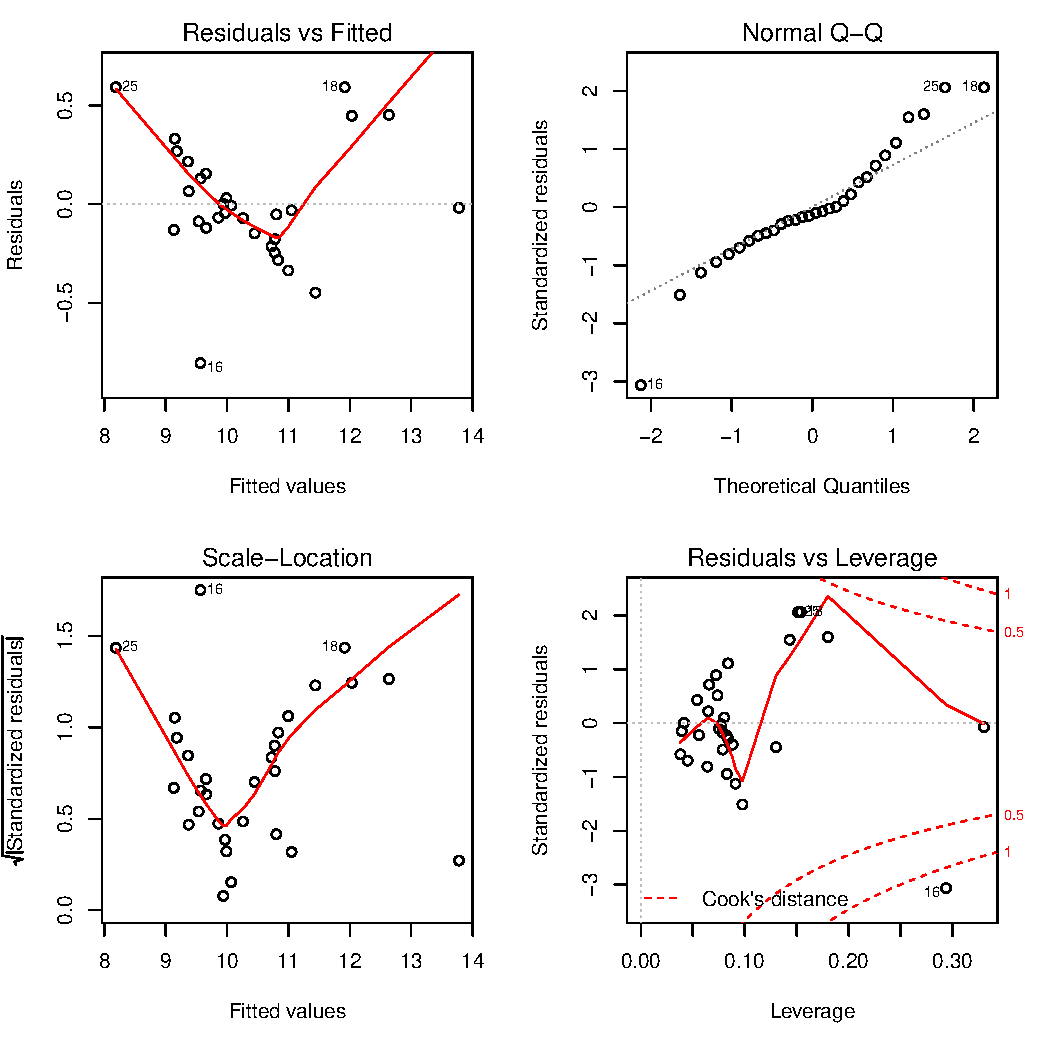
\includegraphics[width=0.6\linewidth]{figure/beamer-unnamed-chunk-26-1} 

}



\end{knitrout}
\end{frame}

%%%%%%%%%%%%%%%%%%%%%%%%%%%%%%%%%%%%%%%%%%%%%%%%%%%%%%%%%%%%%%%%%%%%%%%%%%%%%%%%%%%%%%%%%%%%%%%%%%%%


% %%%%%%%%%%%%%%%%%%%%%%%%%%%%%%%%%%%%%%%%%%%%%%%%%%%%%%%%%%%%%%%%%%%%%%%%%%%%%%%%%%%%%%%%%%%%%%%%%%%%
% \begin{frame}[fragile]{Conclusion}
% \begin{enumerate}
% \item R is a free and open source programming language for statistical computing and graphics.
% \item R contains many useful features for data analysis including data structures such as vectors and data frames that make it easy to perform statistical analysis and visualization.
% \item R is often used for hypothesis testing and understanding how to properly setup and interpret a test is an important skill.
% \end{enumerate}
% \end{frame}
% %%%%%%%%%%%%%%%%%%%%%%%%%%%%%%%%%%%%%%%%%%%%%%%%%%%%%%%%%%%%%%%%%%%%%%%%%%%%%%%%%%%%%%%%%%%%%%%%%%%%
% 

\begin{frame}{Conclusion}
\begin{itemize}
\item Like much of what we cover in this course, the materials reviewed here are to expose you the available tools for data analysis rather than provide all of the ``under the hood" details.
\item If you would like to learn more about the justifications behind using these statistical methods, I would suggest STAT 230 and DATA 311. 
\end{itemize}
\end{frame}





\end{document}

